\section{Architektura}
Na podstawie opisu zidentyfikowano następujące klasy
\begin{itemize}
	\item User
	\item Toolbox
	\item Canva
	\item Model (diagram PERT)
	\item Milestone
	\item Link (połączenie pomiędzy dwoma milestone'ami)
	\item Task (zadania powiązane z danym linkiem)
	\item CriticalPath
	\item Gantt
\end{itemize}

Rysunek~\ref{fig:klasy} przedstawia wstępną propozycję diagramu klas. 
\begin{figure}[h]
	\centering
	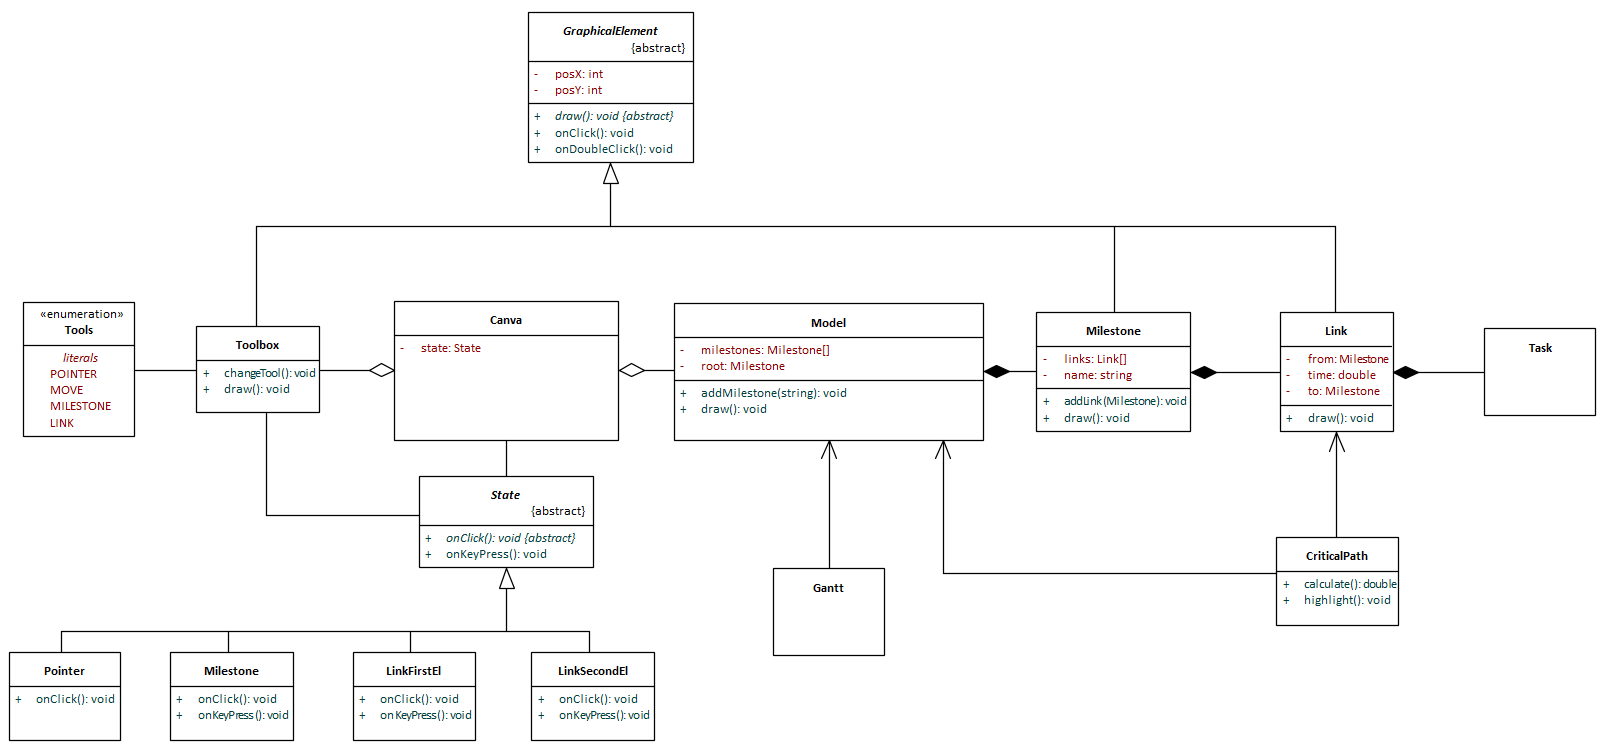
\includegraphics[width=1\linewidth]{img/klasy}
	\caption[Diagram klas]{Diagram klas (pierwsza iteracja)}
	\label{fig:klasy}
\end{figure}

Każdy z elementów, który można narysować rozszeraz klasę \textbf{GraphicalElement}

\subsection{Struktura danych}
Obiekt \textbf{Model} składa się z listy kamieni milowych (obiekty \textbf{Milestone}). Do tego zawiera on wskaźnik na element początkowy (wymagane jest to do obliczania ścieżki krytycznej).

Każdy milestone może być połączony z dowolną ilością innych kamieni milowych, dlatego zawiera on listę obiektów klay \textbf{Link}. Połączenia są skierowane od danego obiektu do innego.

Linki muszą być umieszczone zarówno w źródłowym, jak i docelowym milestone'ie, ponieważ przy przemieszczaniu dowolnego z nich, należy każdy link aktualizować.

W trakcie prac prototypowania rozwiązania stwierdzono, że taka struktura danych nie zapewnia możliwości serializacji (cykliczne odwołania pomiędzy obiektami Milestone, a Link). Zdecydowano się na zmianę struktury danych.

W obiekcie Model zawarto dwie tablice: milestones oraz links zawierające odpowiednio obiekty Milestone i Link. Indeks w tablicy odpowiada za identyfiację danego obiektu. 

Powiązania pomiędzy obiektami zrealizowano przy użyciu tych właśnie indeksów: ich wartości liczbowych zamiast obiektów.

---------------   TODO   ------------------   dodanie nowego diagramu klas   ------------------

\subsection{Maszyna stanu}
\textbf{Toolbox} zawiera stan związany z wybranym narzędziem. Najbardziej skomplikowana (jak do tej pory) operacja to połączenie dwóch milestone'ów - musimy rozróżnić, czy wybrany został już pierwszy z nich, czy już wybrano docelowy. Również musimy sprawdzać, czy źródłowy i docelowy milestone to dwa różne obiekty.

Maszyna stanu została przedstawiona na Rysunku~\ref{fig:fsm-toolbox}

\begin{figure}
	\centering
	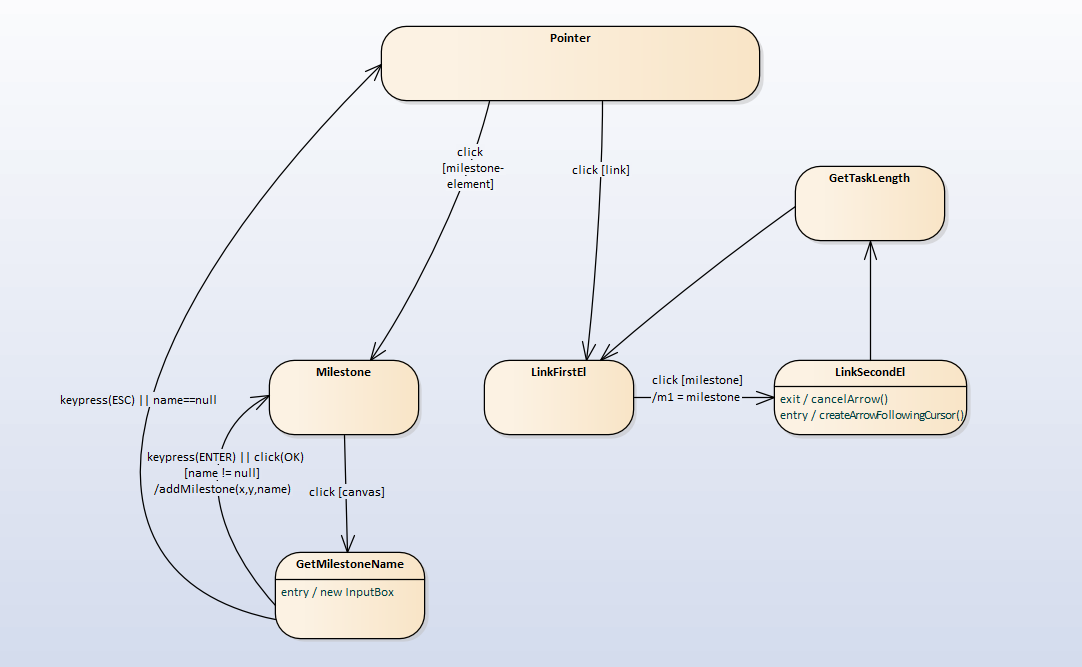
\includegraphics[width=1\linewidth]{img/fsm-toolbox}
	\caption[Maszyna stanu obiektu Toolbox]{Maszyna stanu obiektu Toolbox}
	\label{fig:fsm-toolbox}
\end{figure}